\documentclass[a4paper,12 pt]{report}
\usepackage[utf8]{inputenc}
\usepackage{graphicx}
\usepackage{xcolor}
\usepackage{caption}
\usepackage{subcaption}
\usepackage{float}
\usepackage{amsmath}
\usepackage{listingsutf8}
\usepackage[utf8]{inputenc} 
\usepackage{multirow}
\usepackage{soul}

\usepackage[hidelinks]{hyperref}
\usepackage[bottom]{footmisc}

\usepackage{pgfplots}
\pgfplotsset{width=10cm,compat=1.9}


\usepgfplotslibrary{external}
\tikzexternalize

\usepackage[left=1.1in,right=1.1in, top=1in, bottom= 1in]{geometry}

\usepackage{biblatex} %Imports biblatex package
\addbibresource{biblio.bib}
\definecolor{blu_dmi}{HTML}{002e62}

% \addbibresource{bibliografia.bib
% \pagestyle{plain}
% \setlength{\topmargin}{0.0in}
% \setlength{\headheight}{0.2in}
% \setlength{\headsep}{0.0in}
% \setlength{\footskip}{0.5in}
% \setlength{\textheight}{8.3in}
% \setlength{\textwidth}{6.0in}
% \setlength{\oddsidemargin}{0.5in}
% \setlength{\evensidemargin}{0.5in}
% \setlength{\parindent}{0.4 in}
% \onehalfspacing

\graphicspath{ {images/} }

\title{
{Instagram-inspired attacks to object detection and image segmentation}\\
{\large Università Degli Studi di Perugia}\\
\vspace{25pt}
{
\includegraphics[scale=0.2]{logo.png}}
}

\author{El Assl Youness}
\date{September 2022}

%\renewcommand*\contentsname{Indice}
%\renewcommand{\chaptername}{Capitolo}
%\renewcommand{\figurename}{Figura}
%\renewcommand{\lstlistingname}{Codice}

\begin{document}

% Thesis frontmatter --------------------------------------------

\thispagestyle{empty} %suppress page number

	\noindent % just to prevent indentation narrowing the line width for this line
	
\includegraphics[width=0.15\textwidth]{img/logoUniPg}
	\begin{minipage}[b]{0.7\textwidth}
		\centering
		{\Large \textcolor{blu_dmi}{\textsc{University of Perugia}}}\\
		\vspace{0.4 em}
		{\large \textcolor{blu_dmi}{Department of Mathematics and Computer Science}}
		\vspace{0.6 em}
	\end{minipage}%
	
\includegraphics[width=0.15\textwidth]{img/logoDMI}
	
	\vspace{5 em}

	\begin{center}
		
		{\large \textcolor{blu_dmi}{\textsc{Bachelor's Thesis in computer science}}}
		\vspace{8 em}
		
		{\Huge \textcolor{blu_dmi}{Instagram-inspired attacks to object detection}}
		\vspace{10 em}
		
		\makebox[380pt][c]{\textcolor{blu_dmi}{\textit{Supervisor} \hfill \textit{Student}}}
		\makebox[380pt][c]{\textcolor{blu_dmi}{\textbf{Valentina Poggioni \hfill  Youness El Assl}}}
		
		\makebox[380pt][c]{\textcolor{blu_dmi}{\textit{Co-Supervisor}\hfill}} 
		\makebox[380pt][c]{\textcolor{blu_dmi}{\textbf{Alina Elena Baia}\hfill}}
		
		\vspace{6 em}
		\vfill
		
		\textcolor{blu_dmi}{\rule{380pt}{.4pt}}\\
		\vspace{1.2 em}
		\large{\textcolor{blu_dmi}{Academic year 2021/2022}}
		
		 
		
		
	\end{center}

% ------------------------------------------------------------------

\begin{abstract}
    Object detection is a technology that is used to detect instances of objects in images or videos.
Today this technology is well established and it is applied in numerous territories of image processing, including picture retrieval, security, observation, computerized vehicle systems and machine investigation.
This raises many concerns as we depend more and more from a technology that is still vulnerable to attacks and that can also be used to extract unauthorized information from our data, especially from the images shared on Social Media.

In this work, we propose a black-box adversarial-filter-based attack towards some state-of-the-art object detectors (i.e. YOLO and DETR).
Unlike most adversarial attack techniques found in literature that add small perturbations that cannot be easily detected by human eyes but can be easily recognized by software, our filter composition cannot be distinguished from any other filter composition used extensively every day to enhance photos and images.

    
    

  
\end{abstract}

\tableofcontents

\chapter{Introduction}
Deep Neural Models have established themselves as standard-de-facto technology in most computer vision applications. This is due to the exceptional performances and versatile applicability they demonstrated in the last years. 
However, recent studies demonstrated that these models are susceptible to adversarial examples raising serious doubts on their reliability and trustworthiness, especially when embedded in real world safety and security-critical systems \cite{Szegedy2014IntriguingPO,Goodfellow2015ExplainingAH,Papernot2016TheLO, kurakin2016adversarial} .

Among these researches, the most studied scenario is image classification where the main adversarial objective is to cause system  misclassifications of data by applying some imperceptible image modifications.
In the last years several techniques for adversarial attacks have been proposed in literature. Most of them are settled in the white-box setting where it is assumed that the attacker knows details over the network structure or has access to the gradient values. It is clear that the applicability of such systems is relative low since any attacker cannot assume to have the necessary information \cite{Goodfellow2015ExplainingAH, madry2017towards, kurakin2016adversarial, carlini2017towards,Papernot2016TheLO}.

If we are looking for techniques with a concrete real-world applicability we have to move to the black-box setting. In this case the performance clearly decreases: the attack success rates are in general lower and the modifications applied to the images more visible. Interesting works are the ones proposing unrestricted attacks where the image modifications are not $L_p$-norm bounded: they employ large and visible perturbations while keeping the images realistic, natural looking and non-suspicious. The idea is to obtain images that can admit great differences from the original ones but, without a direct comparison with the original image, they cannot be distinguished from any other real (maybe filtered or edited) image. In this case the objective is not to limit the modifications on pixels but to limit the human perception that a modification has been applied \cite{Colorfool,ACE,wang2021demiguise}.

Extensive efforts have been made to combat these adversarial attacks. Some of them try to find noise, injected patterns and irregularities in the high frequencies image \cite{moosavi2018divide,liao2018defense}, while others try to build robust models adversarially trained \cite{andriushchenko2020understanding,bai2021recent}. 

The problem of achieving realistic attacks and effective defenses becomes more interesting and challenging for more difficult visual recognition tasks including object detection, especially due to their wide applicability to a lot of real-world critical systems such as autonomous driving \cite{feng2021review}, medical imaging \cite{chen2022recent} and smart cities \cite{ahmed2021adapting}. For these tasks,
the number of targets that need to be attacked is much larger
than that in pure classification task \cite{bose2018adversarial}. Moreover, in the case of models implementing the non-maximum suppression module (NMS),  even if a bounding box is successfully attacked, another sub-optimal bounding box may be detected in similar locations. As a matter of fact, it has been shown that existing attack methods primarily designed for classification do not generalize well to object detection \cite{shen2019advspade}. 

Some attack and defense techniques have been introduced in literature but the topic remains largely unexplored, especially in the black-box scenario when only the predicted bounding boxes are accessible to the attacker. Adversarial attacks for object detection were systematically studied for the first time in \cite{xie2017adversarial}.
Then, other approaches have been proposed \cite{arnab2018robustness,liang2021parallel,wang2020adversarial,procNoise_co2019, gu2021adversarial, Lu_2020_CVPR}.  

Another aspect that has not been adequately addressed for object detection is the use of adversarial machine learning techniques as defense methods against private information extraction, especially from images posted on social networks. It has been shown that information can be easily extracted from dataset and learned model in the case of classification \cite{bae2018security,shokri2015privacy,mireshghallah2020privacy,AGV-wiiat}.
In this case having good images without artifacts, patches, or visible noise patterns becomes of primary attention. The use of attacking methods producing good-looking images able to inactivate the information extraction procedures heavily applied on the Web could be of interest for the whole society.\\

In this thesis we propose a new attack method for object detection where the attacks are performed by applying a composition of Instagram-style filters to the image. They are obtained using customized versions of AGV algorithm with multi-objective optimization \cite{agv1} \cite{agv2}. AGV is based on a nested evolutionary optimization technique that can be adapted to several problems acting on the definition of fitness function and targets to optimize. \\
We demonstrate how the AGV evolutionary approach is able to find effective attacks that can overcome the existing ones both in terms of precision and image quality. The main contribution of this thesis can be summarized in: (1) a new method to attack object detection systems producing natural images that can be used also as protection method against unauthorized information extraction on the Web (2) evaluation of the efficiency of our attacks to different object detection models (3) analysis of robustness of two of the most known models (DETR \cite{detr_paper} and different versions YOLO \cite{yolov3, yolov4}). 



\chapter{Background} \label{sec:background}

\section{Adversarial Attacks}
Adversarial attacks are methods to generate adversarial examples that should resemble a valid input for humans but cause a machine learning model to make mistakes.
Their main application is in the field of Computer Vision and in particular image classification, but their applicability has been demonstrated also in other fields. %{\bf[CITARE]}. 

Adversarial attacks can be characterized in several ways. The main one considers the knowledge of the attacker about the victim. \textit{White-box} attacks work by having full access to the model and all its parameters and training details. This was the first case of study, but clearly the assumptions made are too strong to be applied for real-world attacks. 
%%cito esempi attacchi whitebox
\textit{Black-box} attacks, on the other hand, do not have full access to the model and nor to its internal structure.
They only have access to the output for a given input sample.
%%cito esempi di tipi di attacchi blackbox che utilizzando diversi approcci con pro e contro

Moreover, attacks can be classified as {\it restricted} or {\it unrestricted}, considering the amount of modifications they apply to the images in order to fool the systems. 
Restricted attacks generally use a $L_p$-norm distance to bound the modifications. The attacks are crafted with the aim of minimizing the differences between the original image and the adversarial one, even if it means having visible (more or less) artifacts. %In Figures \ref{fig:restricted_tifsgm_adv} and \ref{fig:restricted_sgm_adv}, the attacks produced by \cite{translation_invariant} and \cite{skip-matter}, two of the most recent state-of-the-art adversarial methods, are shown. In both the cases the generated artifacts are clearly visible. \\ 
%\item
Unrestricted attacks use large and visible perturbations while keeping the images realistic, natural looking and non-suspicious. The idea is to obtain images that can admit great differences from the original one but, beyond a direct comparison between the two, they cannot be distinguished from any other real (maybe filtered) image. %In Figures \ref{fig:unrestriced_ace_adv} and \ref{fig:unrestricted_colorfool_adv}, the attacks produced by ACE-Ins \citep{ACE_journal} and Colorfool \citep{Colorfool} are shown. 
The differences between the original image and the adversarial one are in general evident but, looking just at the adversarial one we might not be able to say that it is an attacking image.  
%\end{description}
 
Another aspect that has to be taken into account 
for real-world attacks is the amount of queries to the victim model that are necessary to craft effective attacks. Black-box systems, in general, need a huge amount of queries and, also in the case of systems built to work with limited access to the victim model, several thousands of queries are needed to produce reliable attacks.

\section{Object Detection}
%\subsubsection{Object Detection} 
\textbf{Object Detection} is the task of detecting objects in an image and assign them a label from a certain class. In its general formulation the aim is both to locate and classify multiple objects in a given scene.

Formally, given an object detection model $F$, $x \in \mathbb{R}^{(H \times W \times 3)}$ a 3-channel RGB image $x$ with height $H$ and width $W$ and a list of predefined classes $C$, the object detection output is a list of $M$ objects, each characterized by a rectangular bounding box of vertices $b_i=((x_{0i},y_{0i}),(x_{1i},y_{1i}))$ and a class label $c_i\in C$ as shown, for example, in Fig.\ref{fig:objdet_samples}.


% $F(x) \in \mathbb{R}^{M\times (4+1)}$ s.t. $F(x)=\{(b_i,c_i), i=1,...,M \}$, where $b_i \in \mathbb{R}^4$ is the bounding box for object $i$, $c_i\in C$ is its class label and $M$ is the number of the identified objects.\\


%\subsubsection{Adversarial example on object detection}
\textbf{An adversarial example against object detection}  is an image $x^*$, a modified version of $x$, such that, at least one object (possibly all the objects) recognized in $x$ is not identified or correctly classified in $x^*$. 
This means that $\exists i=1,...,M$, such that either $\nexists j=1,...,M^*\quad  s.t. \quad IoU(b^*_j,b_i) > threshold$ or $ c^*_k\neq c_i \quad \forall k=1,...,M^*\quad  s.t. \quad IoU(b^*_k,b_i) > threshold$, where $IoU(b_j,b_i)$ is the usual \textit{Intersection Over Union} measure used in computer vision between two generic bounding boxes $b_i$ and $b_j$.

% recognized  given  $F(x^*)=\{(b_i^*,c_i^*), i=1,...,M^* \}$
% \begin{equation} \label{eq:advDef_objdet}
%  \quad IoU(b_i^*,b_i) < threshold \qquad \vee \qquad  c_i^*\neq c_i,    
% \end{equation}
% for at least one, but possibly for all, object  
% For each object in the image $x$ the \textit{Intersection over Union} (IoU) between the new bounding box and the original one is under a given threshold or the classification label is different.

\subsection{State-of-the-art models}
The state-of-the-art methods for object detection can be categorized in one-stage and two-stage methods.
One-stage methods only need to go through the network once to locate objects and get their class. The most representative models are YOLO \cite{yolov3,yolov4}, RetinaNet \cite{retinanet}, SSD \cite{ssd} and DETR \cite{detr_paper}.
Two-stage methods treat object detection as a two stage problem: the first stage generates region proposals, including the object's approximate location, while the second classifies and precisely locates the object inside the proposed region. Some of the most famous and best performing two-stage object detectors are Faster R-CNN and Mask R-CNN.



\subsection{YOLO}
 
In this thesis we focus on attacking object detection systems based on YOLO (You Only Look Once) which is a state-of-the-art object detector with real time detection capabilities and high accuracy. 

%“You Only Look Once” YOLO Invented by Joseph Redmon, Santosh Divvala, Ross Girshick, and Ali Farhadi (2015) 
The first version of Yolo was introduced in \cite{redmon2016you} as a model that reframes object detection as a single regression problem to spatially separated bounding boxes and associated class probabilities. 
Over the years different YOLO versions have been released and nowadays YOLOv3 and YOLOv4 are among the most powerful and used models.

\textbf{YOLOv3} uses Darknet-53 to perform feature extraction, %this network as the name suggests ii is composed of 53 convolutional layers with shortcut connections.
a convolutional neural network composed of 53 convolutional layers with shorcut connections.
%\cite{yolov3}
The YOLOv3 algorithm first separates an image into a grid. 
Each grid cell predicts some number of anchor boxes around objects that score highly with the set of predefined classes.
This procedure can result in several overlapping bounding-boxes that are later corrected using Non-Max Suppression (NMS).
NMS is performed selecting the box with the highest score, calculating the interval overlap of this box with other boxes and omitting the boxes that overlap significantly.
To know which boxes overlap significantly it uses the measure of IOU (Intersection over Union): the greater the region of overlap, the greater the IOU.

\textbf{YOLOv4} is an improvement of the Yolov3 algorithm obtained by expanding the  Bag-of-Freebies (BoF) feature list that increases the detector accuracy without affecting the speed, like for example the use of genetic algorithms for
selecting the optimal hyperparameters, the use class label smoothing for sigmoid activation and the use of Cross mini-Batch Normalization, and many others. Authors showed to reach a mAP increment of 10\% increasing the processed  frames per second (FPS) by 12\%.

\subsection{DETR}
\textbf{DETR} (\textbf{DE}tection \textbf{TR}ansformer) is a new technique introduced by the Facebook research team in an article titled "End-to-End Object Detection with Transformers", presented in 2020 \cite{detr_paper}.
It’s a new object detection model created using Transformers architectures generally used in NLP.\\

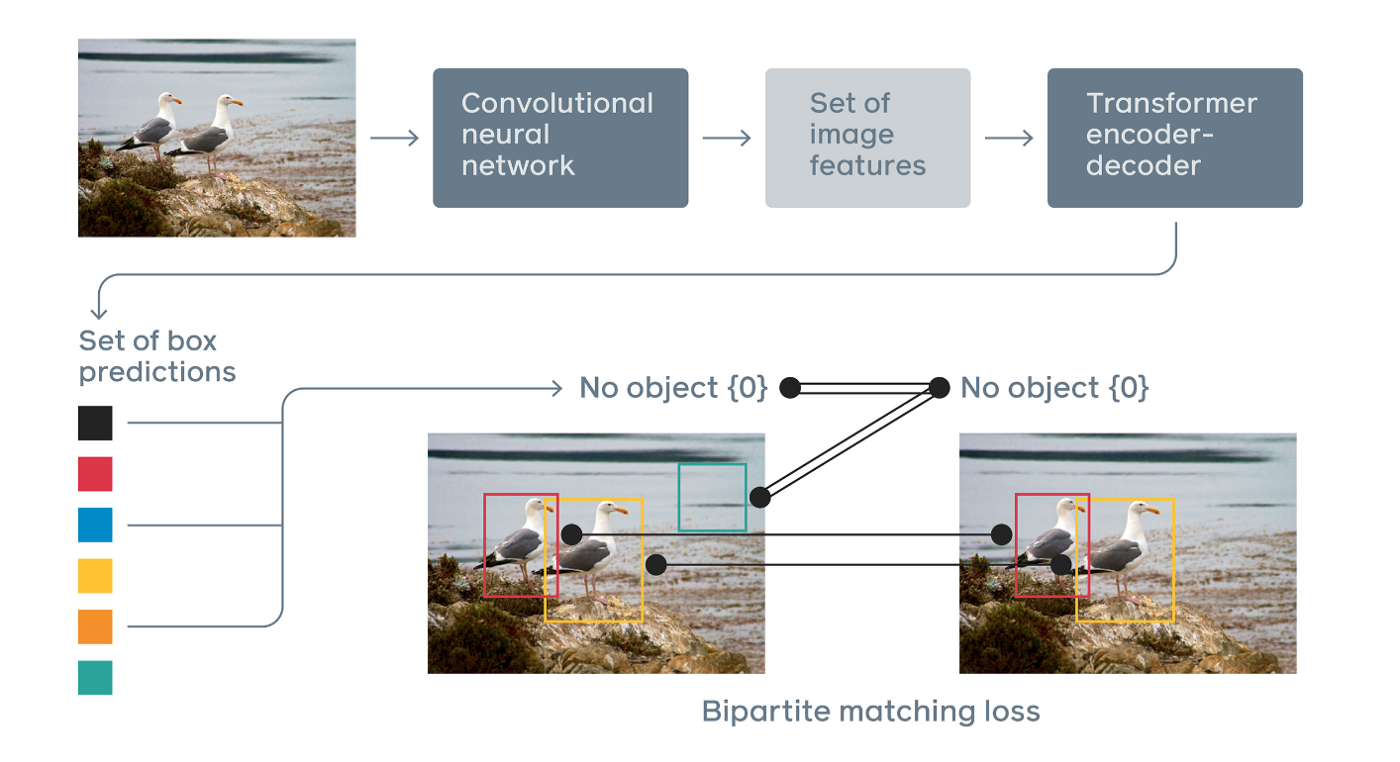
\includegraphics[width=\textwidth]{Introduzione/imgs/detr_architecture.png}\label{fig:detr_architecture}
As shown in (fig: \ref{fig:detr_architecture}) DETR directly predicts (in parallel) the final set of predictions by combining
a CNN with a transformer architecture. \\During training, bipartite matching
uniquely assigns predictions with ground truth boxes. Prediction with no match should
return a "no object" class prediction \cite{detr_paper}.


DETR is fast thanks to this parallel processing capability and for the fact that it doesn't use restrictive techniques such as anchor boxes and NMS, but it requires a lot of gpu memory compared to the other tested models.

It reaches very good performance, both in terms of  accuracy and run-time, very similar to the well-established and highly-optimized Faster RCNN baseline on the COCO dataset.
DETR achieves 42.0 AP computed on COCO 2017 val5k, with 0.036s inference time evaluated over the first 100 val5k COCO images.

\chapter{Related Works} \label{sec:related}
Recently, different algorithms have been proposed to craft 
adversarial attacks against object detection.

Adversarial attacks for object detection are systematically studied for the first time in \cite{xie2017adversarial} with the algorithm DAG. The authors proposed an iterative white-box method that tries to assign adversarial labels to each RoI in the image adding noise to the original image. It runs gradient backpropagation to minimize a loss function computed as the sum, with respect to all the targets in the image, of the differences between the score assigned to the original correct class and the one assigned to the adversarial incorrect class.

Co et al. proposed in \cite{procNoise_co2019} to create attacks to object detection systems by applying procedural noise functions, in particular Perlin noise and Gabor noise, to the original images. They hypothesized that procedural noise, which exhibits patterns visually similar to the Universal Adversarial Perturbations (UAPs) proposed by \cite{MoosaviDezfooli2017UniversalAP}, can also act as UAPs. They empirically demonstrated the vulnerability of some Deep Convolutional Networks to this procedural noise, parameterized by Bayesian Optimization, for the classification task on the ImageNet dataset. Then, they demonstrated that the same procedural noise is able to attack also Yolo v3 object detector on the dataset MS COCO.

In \cite{wang2020adversarial} the authors represented the black-box attack problem as an optimization problem in the manifold of sample images, and then designed a GA-PSO algorithm to solve the problem and generate adversarial examples. In particular they create the image particle swarm with attacking images generated as randomly (heavily) noised version of the original image and then try to optimize their quality moving them towards the original image.

We have to note that all the methods described above share the same general structure: optimized noise added to the original images in order to obtain effective attacks. They differ on the noise applied and on the optimization algorithm used but the high level idea is the same. Moreover, all of them create restricted attacks since they control the modifications on the images by means of $L_p$-norms.  

Our work falls in the same category but with significant differences: we craft the attacks as compositions of Instagram-inspired filters (instead of noise) and we optimize them by means of a nested evolutionary algorithm. This algorithm combines GA (genetic algorithm) to obtain the composition and ES (evolution strategy) to optimized the parameters of the filters. Moreover, we use a multiobjective optimization approach that can take into account different conflicting objectives such as the minimization of mAP or IoU and the maximization of the image quality. The application of non limited filters and the image quality assessment in the multi-objective optimization process allow us to create unrestricted attacks able to produce image artifact-free that appear more natural than the ones produced by the other methods. The differences between attacking images produced applying the procedural noise proposed in \cite{procNoise_co2019} and the ones produced by our algorithm can be observed comparing the images in Figures \ref{fig:objdet_samples}--\ref{fig:procnoise_samples} where examples of attacking images produced by our method (Fig. \ref{fig:objdet_samples}) and procedural Noise method (Fig. \ref{fig:procnoise_samples}) are shown. The patterns produced by procedural noise are evident.

Another class of adversarial attacks to object detection includes the methods that transform white-box attacks into black-box attacks exploiting their transferability across different models. In case of high transferability, white-box  methods can be used in a black-box setting transferring the attacks found for a given known model towards an unknown model. 

In \cite{liang2021parallel} the authors showed that optimizing rectangular perturbations (using a white-box method against a given model) on regions having higher probability to contain objects provides effective attacks to object detection systems that use different DNN as backbone.  

An interesting exception is represented by the \textit{Dispersion Reduction} method proposed in \cite{Lu_2020_CVPR}. The authors' idea is to transfer the concept of image "contrast"  into the feature maps produced by a convolutional neural networks. As lowering the contrast of an image can make the objects depicted unrecognizable, they proposed to reduce the contrast of an internal feature map to degrade the object detection. They formally defined the problem as a minimization problem of the dispersion (they use standard deviation) of the intermediate feature map of the modified image constrained by the $L_\infty$-norm with respect the original one.

\chapter{The Algorithm} \label{sec:algorithm}

In this thesis we extend the AGV method previously proposed in \cite{AGV-evoapps,AGV-wiiat} to craft adversarial attacks against methods for object detection. The core algorithm is structured as a nested-evolutionary algorithm which finds an optimal unrestricted adversarial perturbation by composing and optimizing multiple image filters. The algorithm consists of two optimization steps: given a predefined set of popular image filters, the outer optimization phase focuses on finding a sequence of filters to apply to the image, while the inner step optimizes the parameters of these filters to obtain the attack. The core algorithm is described in Algorithm \ref{agv_core} and details on the algorithm components are provided in the next sections.

%\noindent The structure of the core algorithm is reported in Algorithm 1.
% \begin{figure}[h] \label{fig:AGV_alg}
% \centering
% \includegraphics[width=0.7\textwidth]{agv_core_algorithm.PNG}
% \caption{AGV core algorithm}
% \end{figure}

\begin{figure}[]
\centering
    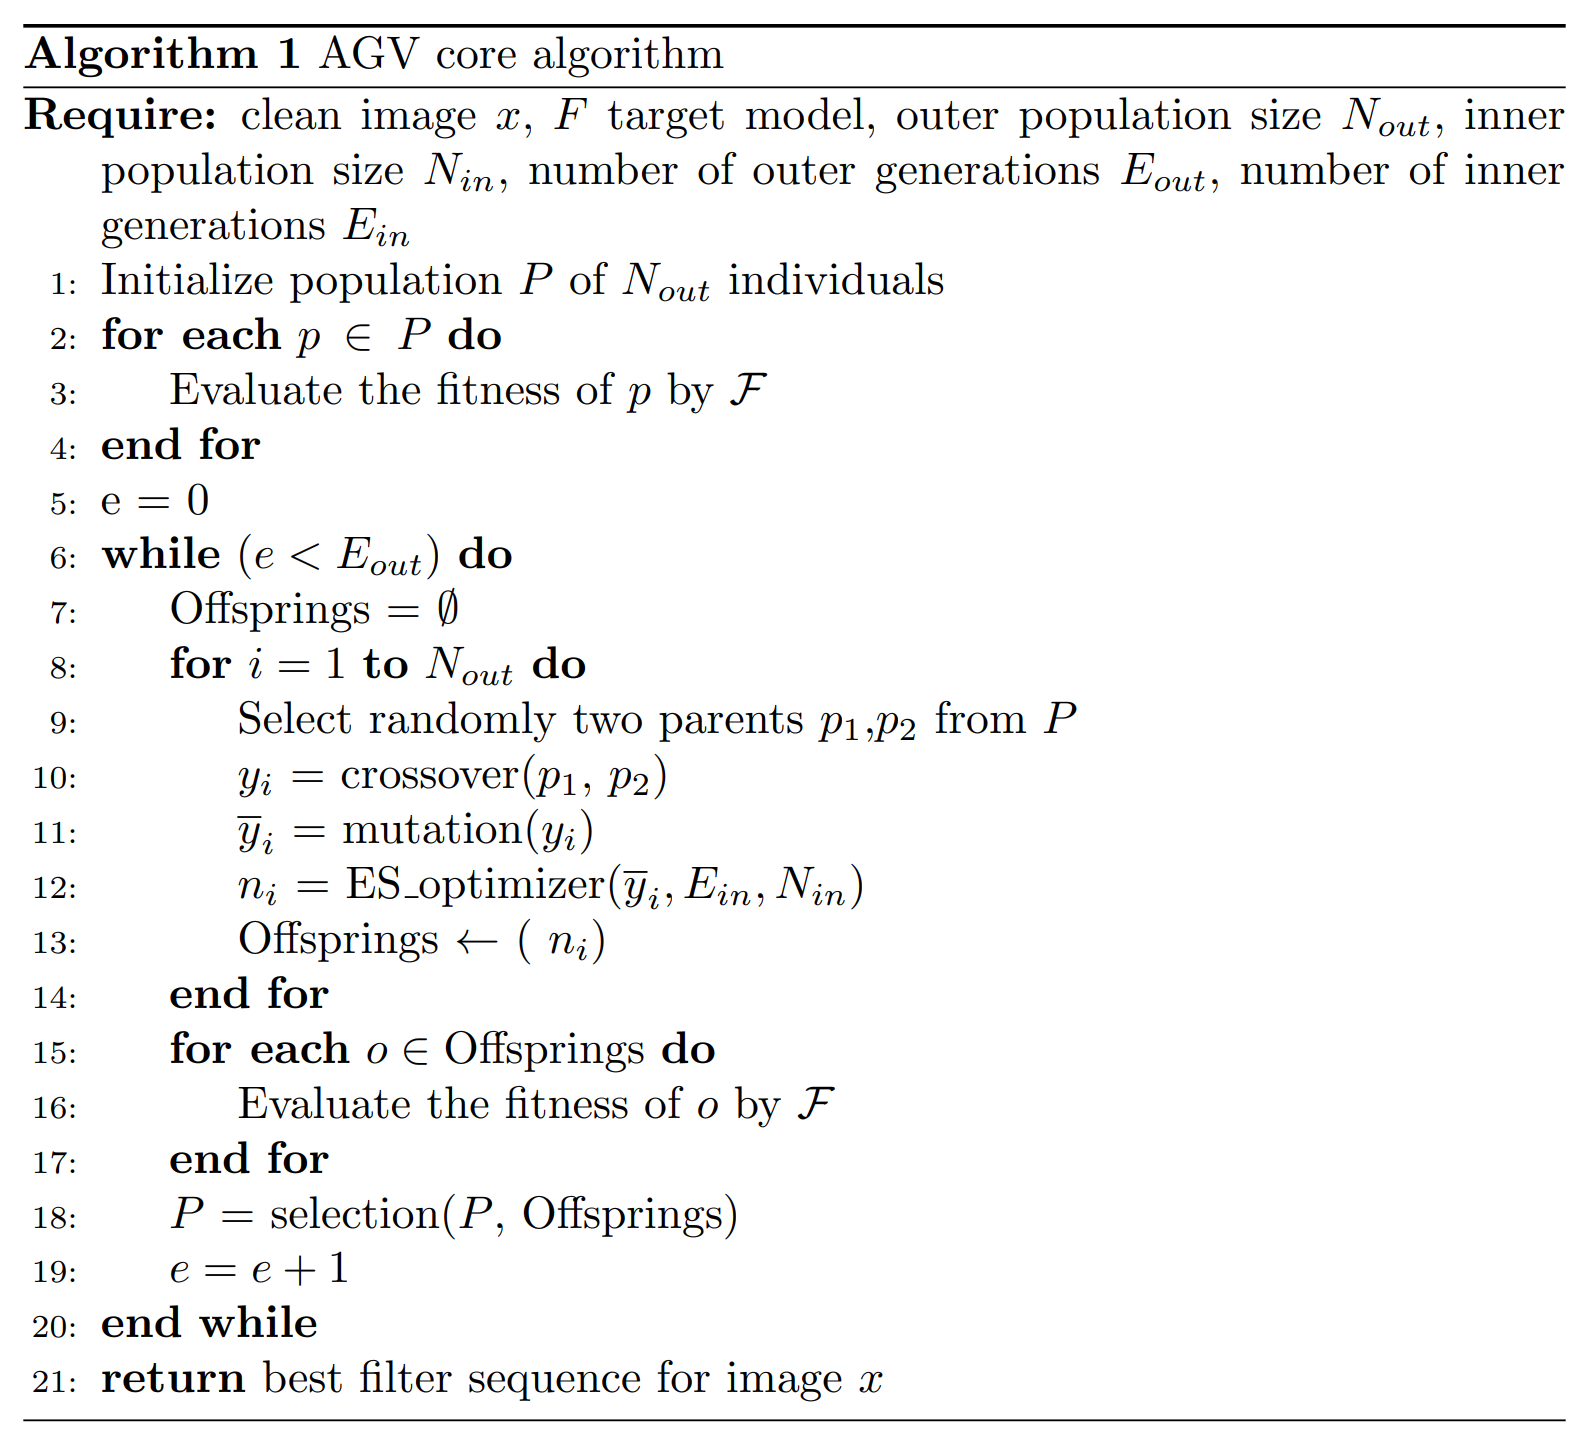
\includegraphics[width=1.0\textwidth]{Attack/charts/agv_alg.png}
    \caption{}
    \label{agv_core}
     
      %\caption{Normal Case: 1 Request \& 1 Response.}
\end{figure}

\section{General Problem Definition}
Given a set $S = \{ f_1, f_2, \dots, f_m \}$ of Instagram inspired image filters, and a clean image $x$, we want to find a sequence of $n$ parametrized filters $\{f_{k_1}(\alpha_1,s_1),\ldots,f_{k_n}(\alpha_n,s_n)\}$ able to produce an adversarial attack against the victim model $F$ such that 
 \begin{equation}      
 \begin{array}{cc}
      x^* = f_{k_n}(\alpha_n,s_n)(\dots f_{k_2}(\alpha_2,s_2)(f_{k_1}(\alpha_1,s_1)(x)))\\
      x^* = \mathrm{argmin} \; ODP(F(x^*))
      
 \end{array}
    \label{eq:filter_application}
 \end{equation}
 where $ODP$ is a measure of the Object Detection
Performance.
Specific definition of $ODP$ is provided in the following Sections \ref{sec:objdet}.
 

\section{Image Filters}

The unrestricted adversarial perturbation is inspired by the popularity of Instagram filters and their ease of use. In particular, commonly-used well-known image filters are employed in order to alter  different features of an image, such as contrast, saturation, brightness, etc. Such image manipulations are able to generate a variety of editing styles, ranging from more vivid and bright colors to more soft and warm looks. The implemented filters are Clarendon, Juno, Reyes, Gingham, Lark, Hudson, Slumber, Stinson,
Rise, and Perpetua.
Each filter modifies an image with respect to different aspects and each filter is parameterized by two main parameters that the inner algorithm has to optimize: intensity $\alpha$ and strength $S$.

The parameter $\alpha$ controls the level of intensity of each basic feature of the filter implementation, like saturation, brightness, contrast, gamma correction and so on. On the other hand, we define the parameter $s$ as the parameter of the convex interpolation between the original image $x$ and the its filtered version $x^*$ that allows us to control the strength of the filter application.
\begin{equation}
strength(x,x^*,s) = (1.0-s) \cdot x + s \cdot x^*
\end{equation}

where in the case of $s=0$ the image remains unaltered, while with $s=1$ the filter function applies the maximum allowed manipulation and returns the filtered image $x^*$.\\

\noindent \textbf{Image Quality Assessment}: Heavy applications of multiple filters can create unnatural looking images which cannot bypass a human judgement. Therefore, in order to keep the aesthetics, naturalness and distortions within acceptable parameters, we employ the \textit{Structural Similarity Index Measure} (SSIM), that is a method for predicting the perceived quality an image. SSIM, introduced by Wang et al. \cite{SSIM}, is a well-performing and widespread Full-Reference method (meaning that it requires a reference image to compute the quality score) that is able to automatically evaluate the quality of the adversarial examples generated by the algorithm. SSIM is a context-aware metric that measures the image degradation as perceived changes in the structural information. Structural information represents the structure of objects in an image which are independent of contrast and luminance. Therefore, SSIM is defined as a comparison function of contrast, luminance and structure computed over the image. By design, the metric satisfies the symmetry, boundedness and unique maximum property that assures an upper value of 1 if and only if the two images compared are identical. In practice, a score higher than 0.99 indicates that the images are indistinguishable. 



\section{Outer optimization}
We employ a genetic algorithm for the outer optimization step where a population of $N$ candidate filter combinations is evolved towards an optimal solution.
%A new generation is created by altering and mutating 
%The genetic operators are applied in order to breed a new generation: 
To create a new generation, randomly selected individuals are altered and mutated by means of the genetic operators, such as crossover and mutation. Then, a problem-specific fitness function is used to measure the quality of each candidate and only the $N$ fittest solutions are selected and passed onto the next generation.

%\noindent The main algorithmic steps are the following:
\begin{itemize}
    \item {\bf Initial Population}: each individual is generated by randomly choosing a predefined number of filters with both parameters set to 1. 
    \item { \bf Crossover}: the generation of new off-springs is handled by a standard one-point crossover operation where the genetic information from 
    a pair of randomly selected candidates is combined in order to produce a new solution. Thus, the off-spring will share genetic characteristics with both parents along with their optimized parameters.
    \item {\bf Mutation}: is applied in order to maintain genetic diversity from one generation to another. It consists of replacing a filter from a sequence with another one based on a probability mutation. Moreover, in this case, the substituent filter is initialized with random parameter values in order to perform mutation over the parameters as well.
    \item {\bf Selection}: at the end of each generation, a fitness-based selection process is used to pick the $N$ fittest individuals from the set composed of parents and off-springs having size $2N$. 
    %The above mention steps (with except of initialization) are repeated  until a termination criteria is met, i.e. the algorithm reaches the allowed number of generations. 
    In particular, since one of the aims of this work is to create natural looking, artifacts free adversarial samples, we incorporate into the selection process both a measure of the attacking ability and an image quality metric. Therefore, the selection process is defined as a multi-objective optimization problem where we want to minimize the performance on the task  \textit{Object Detection Performance (ODP)}  while $SSIM(x, x^*)$  is maximized. Thus, the multi-objective fitness function to minimize is formulated as:
    \begin{equation} \label{eq:general_fitness}
       \mathcal{F}(x,x^*) = \{ ODP(x^*), 1-SSIM(x, x^*)\},
    \end{equation}
    where $x$ is the original image, $x^*$ is the modified image according to (\ref{eq:filter_application}), 

 and $SSIM$ is the metric used to control the applied perturbation. The multi-objective problem is handled by the non dominated sorting and crowding distance NSGA-II algorithm \cite{NSGA-II}.
\end{itemize}

\section{Inner optimization}

The parameter optimization is managed by means of $(1,\lambda) $ Evolutionary Strategy.
In particular, this algorithm evolves a population of lists of parameters for every individual in the outer algorithm. For each inner individual batch, $\lambda$ samples are created by perturbing the original individual. ES uses the fitness values of the batch samples  to estimate a gradient towards a better solution.  The gradient value is then used to update the original individual. This  process is performed over multiple iterations. 

\section{Allowed Queries}
An important aspect that has to be taken into account 
for real-world attacks is the amount of queries to the victim model that are necessary to craft effective attacks.
This is important because it is strictly related to the possibility of being intercepted by defense mechanisms that can be implemented to protect the victim model.

Our algorithm works with limited accesses to the victim model that is called every time we have to compute the fitness function. Besides the explicit calls to the evaluation function made in the initialization step and in the last step of each outer iteration, we have to consider the $E_{in}\times N_{in} $ calls made by the inner optimization phase (filters' parameters optimization) for each element in the outer population. 
Hence, the maximum number of allowed queries can be easily computed as: 
\begin{equation} \label{eq:queries}
   Q_{MAX} =  N_{out} + E_{out} \times ( N_{out} \times  E_{in} \times N_{in} + N_{out}),
\end{equation}
where $N_{out}$ is the size of the outer population, $N_{in}$ is the size of the inner population, $E_{out}$  is the number of outer generations, and $E_{in}$ is the  number of inner generations.





\section{AGV Attacks on Object Detection} \label{sec:objdet} 
%punti di differenza rispetto all'alg originale
In order to apply AGV algorithm to Object Detection we have to define the fitness function used by the algorithm to guide the search.
The fitness function for Object Detection uses, besides SSIM as described in (\ref{eq:general_fitness}), the function ODP (Object Detection Performance) as implementation of Task Performance function, hence
$$\mathcal{F}(x,x^*) = \{ ODP(x,x^*), 1-SSIM(x, x^*)\}$$
%TP evaluates the performance of the model on a given image (X) in which we applied the proposed filters (Xf). This is done to approximate the optimal ones and their parameters in order to minimize the performance of the model in X.

To compute $ODP$, we paired each bounding-box detected in the original image $x$, i.e. each $b_i$ in $F(x)$, with ones detected in the perturbed image $x^*$, i.e. $b^*_i$ in $F(x^*)$, having the same label $c^*_1=c_i$ and $IoU> 0.5$.
For each pair, ODP is increased by $IoU(b_i,b^*_i)/\vert F(x)\vert$, so that the performance is the weighed sum of the $IoU$ of the paired boxes with respect the total number of boxes in the original image.
Minimizing this function allows us to fool the model into getting the wrong classification (raise the misclassification rate) and to lower the $IoU$ values below the threshold. The algorithm is proposed  in Algorithm \ref{algODP}.



\begin{figure}[ht]
\centering
    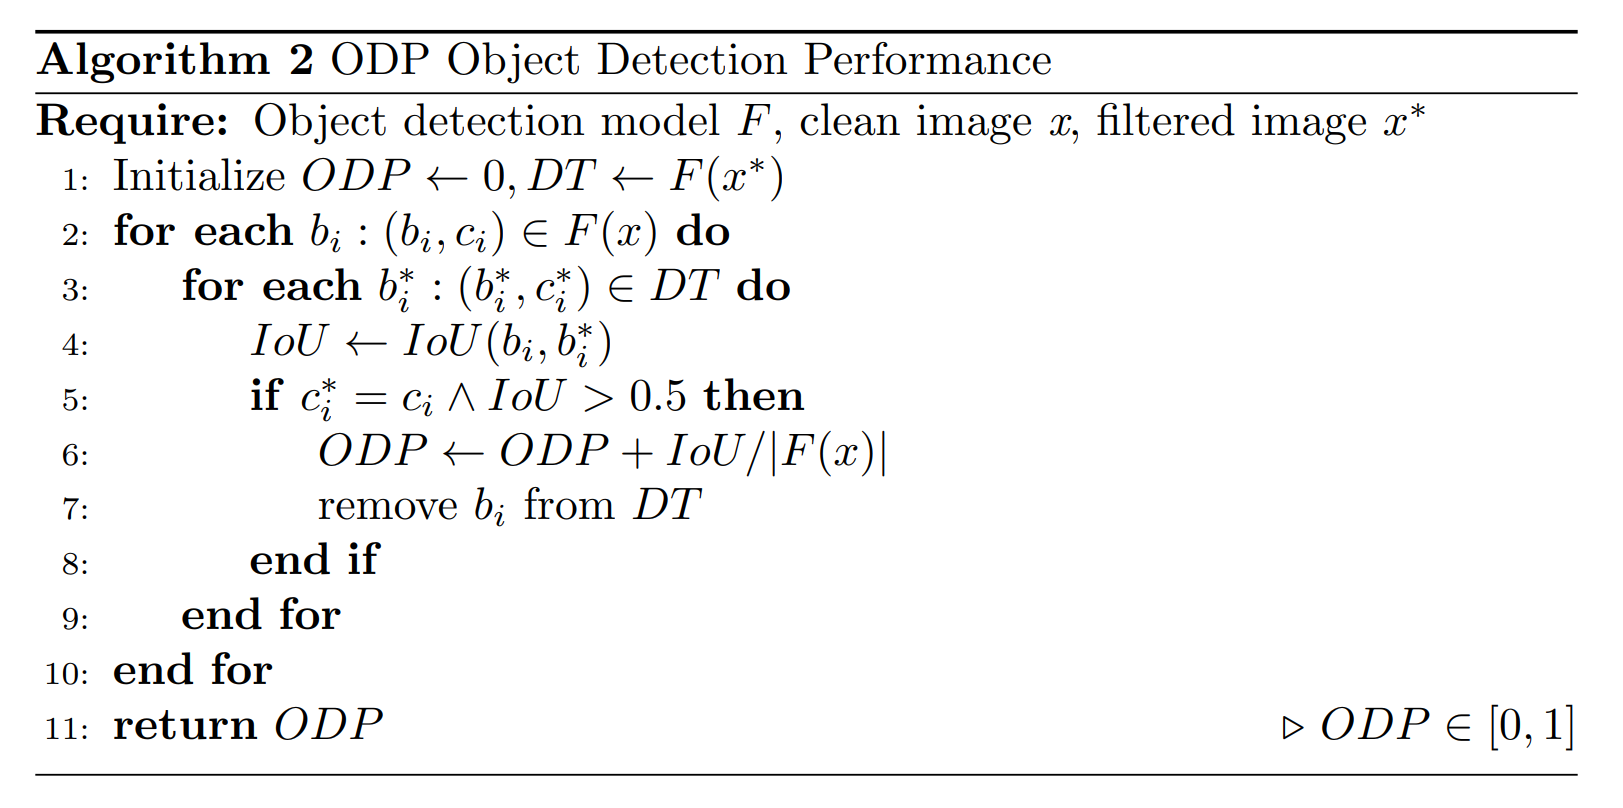
\includegraphics[width=1.0\textwidth]{Attack/charts/odp_alg.png}
    \caption{}
    \label{algODP}
     
      %\caption{Normal Case: 1 Request \& 1 Response.}
\end{figure}

% Given $Xf$ an image derived from the clean one by applying a sequence of filters, $Y$ the bounding-boxes predicted by the model on the clean image $X$, the Object Detection Performance (ODP) function is evaluated by the following:
% \begin{equation}
% %\begin{aligned}
% %\resizebox{.8\hsize}{!}{
%     ODP(Xf,Y)=\sum_{i=1}^{len_y} 1/len_y \sum_{j=1}^{len_x} IOU(y\_bbox_i,x\_bbox_j)      [label(y\_bbox_i)=label(x\_bbox_j) \wedge IOU(y\_bbox_i,x\_bbox_j)]
% %\end{aligned}
% %\normalize
% \end{equation}
% with $y\_bbox \in Y$ and $x\_bbox \in model.predict(Xf)$.


\chapter{Experiments} \label{sec:experiments}
Several experiments were run in order to evaluate the effectiveness of our attacks against different models of object detection and semantic segmentation, as well as to investigate the behaviour of the algorithm with respect to the number of filters applied. Moreover, comparisons with other state-of-the-art methods are provided. 
Finally, we studied the efficiency of the algorithm in terms of number of queries needed to attack the model and about the quality of the images obtained.
1
 


\section{Object Detection}
\subsection{Experimental Setup} \label{sec:ExpSetUp_objdet}
\textbf{Dataset}: We randomly selected 400 images from the MS COCO Val2017 dataset. It is a large-scale dataset extensively used for training, testing and evaluating the performance of object detection models. It contains 80 object categories, such as person, car, bird, and many more. \\


\noindent\textbf{Attacked models}: The target models chosen to test AGV for object detection are DETR \cite{detr_paper} and YOLO \cite{yolov3} \cite{yolov4}. 

Recent studies have shown that the YOLOv3 model \cite{yolov3} is one of the most robust object detector against adversarial attacks \cite{Lu_2020_CVPR}. Therefore we have chosen this model as target in order to test the capabilities of our proposed method. This choice also facilitates the comparisons with other models since it is one of the most used models in literature. Moreover, since the new version YOLOv4 was recently presented \cite{yolov4}, we decided to analyze if also model robustness is increased with respect to the previous version. Finally, since the tiny versions of YOLO are famous models proposed to run on embedded systems with low capacity and computation capability and IoT-based architectures, we think it is interesting to assess the robustness of these model too. 
In particular we wanted to examine if the differences in complexity and architecture of these models are also related to the their robustness against adversarial attacks.

To the best of our knowledge, the robustness of these models to adversarial attacks has never been studied. To run the experiments, we used publicly available pretrained networks provided in the official repository
\url{https://github.com/pjreddie/darknet}, standard settings with input dimensions 608 x 608 x 3 for YOLOv3, YOLOv4 and 416 × 416 × 3 for YOLOv3-tiny, YOLOv4-tiny and an IOU threshold of 0.5. 

Moreover, we decided to use DETR as a target model, because it is a very recent model using transformers, one of the best object detector models in terms of mAP, that even outperforms the well established Faster-RCNN \cite{detr_paper}.

%In our case we chose ResNet-50 as model for the backbone layer 
%Non scrivo che usiamo ResNet-50 perché già in DETR R50 "R50" sta per ResNet-50
We used the implementation of DETR R50 referenced by its paper \url{https://github.com/facebookresearch/detr} with the pretrained weights loaded via torch hub.\\
\\

\noindent \textbf{Hyperparameter configuration}: 
The AGV algorithm was configured as follows: population size $N_{out}=10$, for the outher algorithm, generations $E_{out}=3$ and a mutation probability $\rho= 0.5$; for the inner algorithm the population size $N_{in}=5$, the number of generations $E_{in}=3$, initial learning rate = 0.1 and decay rate = 0.75. Experiments were run with $nf = 3,4,5$ filters.  These values are the result of a preliminary experimental phase conducted  to find a good trade-off between performance and computational time.\\

\noindent \textbf{Metrics:}
We use \textit{precision}, \textit{recall}, and \textit{mean average precision} (\textit{mAP}) as our primary metrics to evaluate the performance of the models before and after the adversarial attacks.
Precision and recall are the usual measures, used also in the image classification task, able to measure how accurate predictions are, while 
\textit{mAP} is the main metric used to evaluate object detection models.

The general definition for the Average Precision (AP) is finding the area under the precision-recall curve.
\begin{equation}
p = \frac{TP}{TP+FP} \hspace{0.4cm}
r = \frac{TP}{TP+FN} \hspace{0.4cm}
AP= \int_{0}^{1} p(r)dr
\end{equation}

The mean Average Precision or mAP score is calculated by taking the mean AP over all classes and over all IoU threshold.

For the COCO 2017 challenge, the mAP is averaged over all object categories and 10 IoU thresholds (IoU from 0.5 to 0.95 with a step size of 0.05).
mAP\_75 and mAP\_50 are also usually used in evaluating object detection models where 50 and 75 represent the respective IoU thresholds.

We use the COCO definition of mAP where a 101-point interpolated AP definition is used.





%AGV parameters: number of filters 3,4 and 5, number of images 400, population size 10, epochs 3, batch size 1, params optimizer "ES", params strategy "direcs", params pool "offsprings", selection "pareto", distance function "SSIM", repetitions True  

\subsection{Results}
The performance of our method has been firstly evaluated analyzing the decrease in terms of \textit{mAP, mAP\_75 and mAP\_50} obtained on the dataset described in Section \ref{sec:ExpSetUp_objdet} by varying the number of filters.  

In Figure \ref{hysto_objDet} the distributions of \textit{mAP\_50} values for all the models tested are reported. Blue columns stand for values obtained testing clean images, while orange columns stand for values obtained testing images respectively with 3, 4 and 5 filters. Comparisons with respect the models can be made reading the columns, while comparisons with respect the number of filters applied to the images can be made reading the rows.

From the histograms we can easily see how the distribution of all the \textit{mAP\_50} values shift towards lower values in the case of filtered images. In particular for all the combinations, the number of images with the highest \textit{mAP\_50} values  significantly decrease (blue columns in the right part of each plots is significant higher than the orange ones), while the number of images having the lowest \textit{mAP\_50} values significantly increase (orange columns in the left part of each plots is significant higher than the blue ones); and the differences widen as the number of filters increases. 

\begin{figure}[h] 
\centering
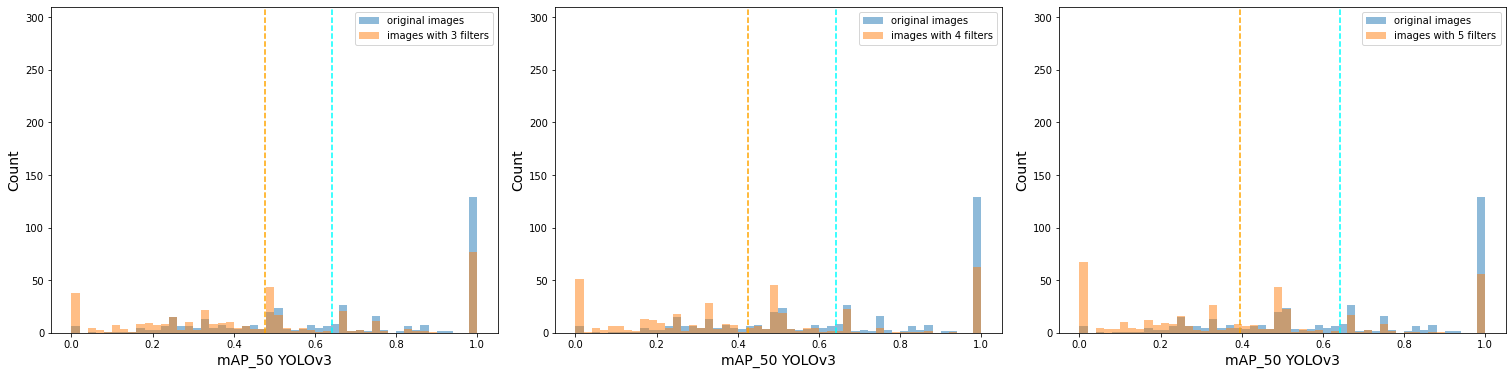
\includegraphics[width=1\textwidth]{Experiments/imgs/y3.png}
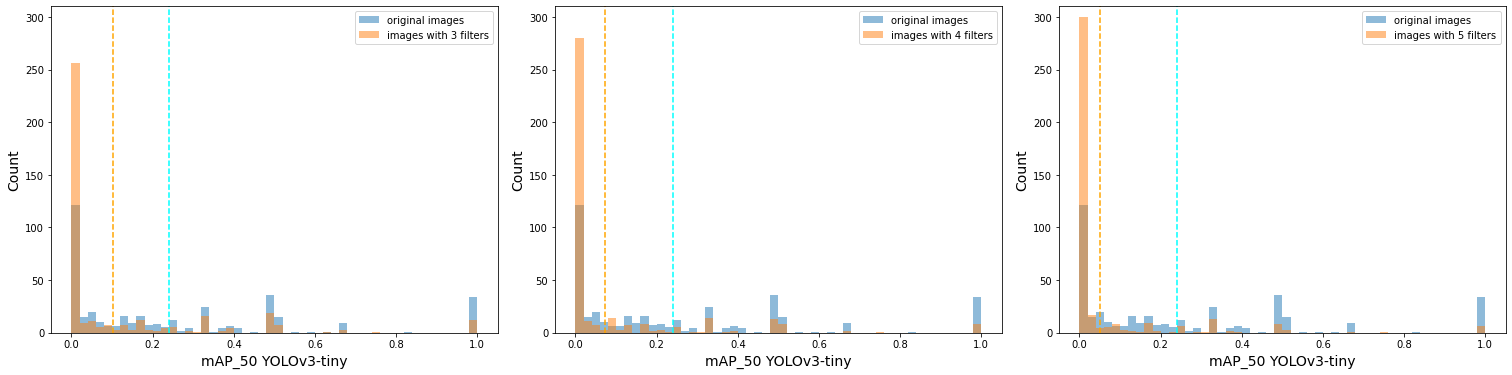
\includegraphics[width=1\textwidth]{Experiments/imgs/y3t.png}
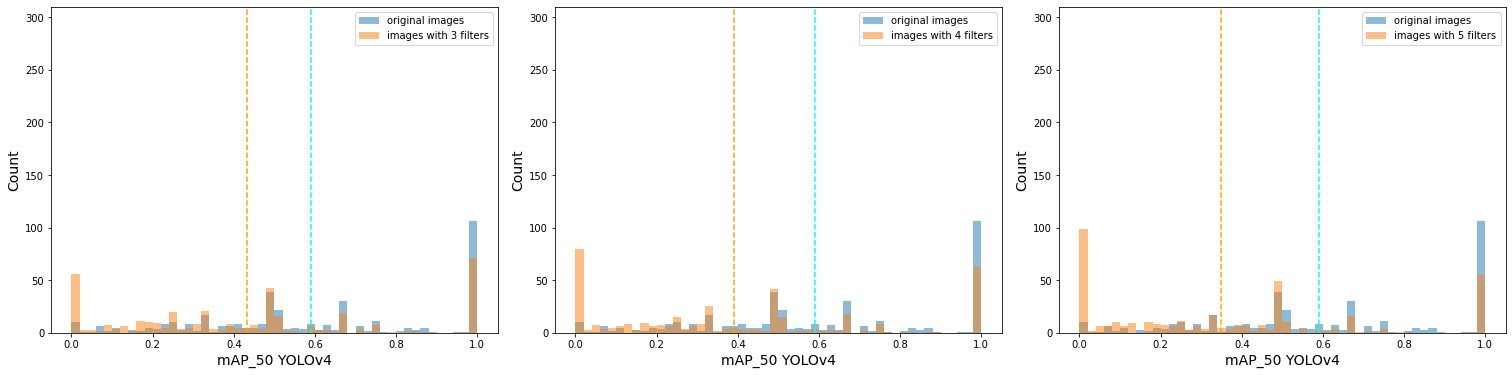
\includegraphics[width=1\textwidth]{Experiments/imgs/y4.png}
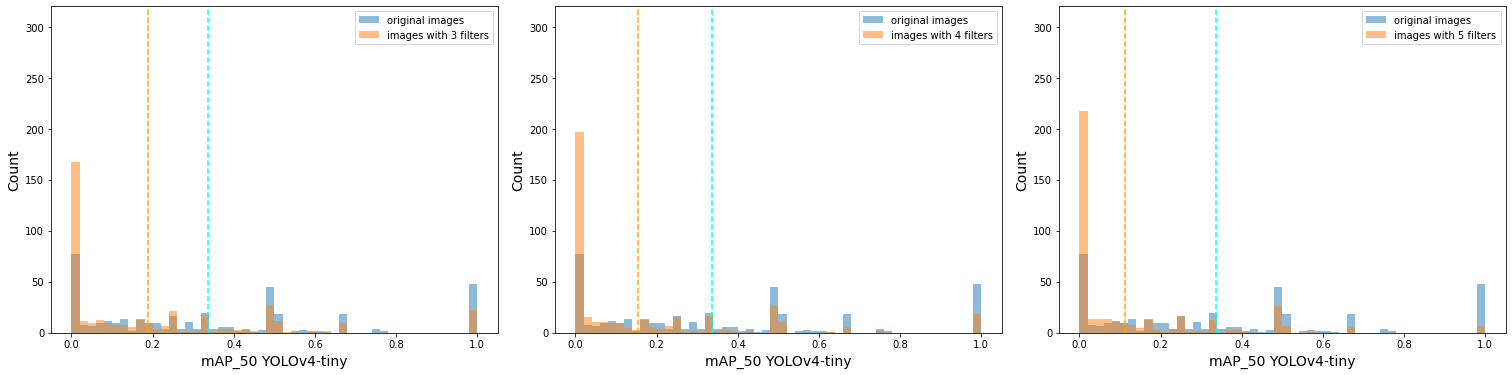
\includegraphics[width=1\textwidth]{Experiments/imgs/y4t.png}
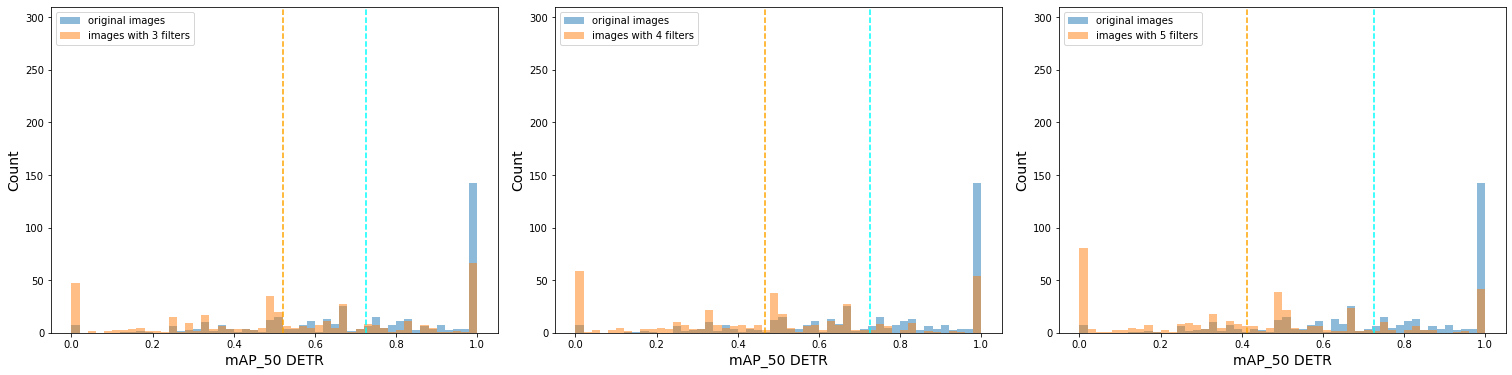
\includegraphics[width=1\textwidth]{Experiments/imgs/detr.png}
\caption{Distribution of AP\_50 values obtained on YOLOv3, YOLOv3-tiny, YOLOv4, YOLOv4-tiny, DETR. The vertical blue dotted line represents the mean over all the mAP\_50 values of the original images. The orange one represents the mean over all the mAP\_50 values of the filtered images}
\label{hysto_objDet}
\end{figure}


If we observe the number of images where all the objects disappear (mAP\_50=0 can be effectively taken as an additional measure for the model robustness) as we espect, besides the mAP\_50 value on 3 filters, YOLOv4 confirms to be the most robustness model and as we expected, both the tiny versions present an impressive robustness decrease with respect their original version. 

An unexpected result can be seen on the decrease of the mAP value in DETR, despite being the best performing model on the clean dataset, the combination of 5 filters decreased its mAP by 53\%.

This behaviour can be observed also analyzing the Precision values in Table \ref{tab_objDet}.


\begin{table}[H]\caption{YOLO and DETR Attack results. Precision and Recall values are calculated with IOU threshold 0.5.\\
In BRISQUE, the lower the score, the better the image quality should be (↓). \\In NIMA, the higher the score, the better the image quality should be (↑).}
\centering
\resizebox{\textwidth}{!}{%
\label{tab_objDet}
\begin{tabular}{llllllllll}
\hline
\multicolumn{10}{c}{\textbf{YOLOv3}} \\ \hline
 & mAP & mAP\_50 & mAP\_75 & precision & recall & SSIM↑ & NIMA↑ & BRISQUE↓ &  \\ \cline{2-9}
no filters & 0.32 & 0.51 & 0.35 & 0.53 & 0.53 & 1.00 & 5.07 & 51.49 &  \\
3 filters & 0.22 (-30\%) & 0.35 & 0.25 & 0.24 & 0.35 & 0.86 & 4.77 & 56.18 &  \\
4 filters & 0.21 (-36\%) & 0.32 & 0.23 & 0.21 & 0.32 & 0.83 & 4.76 & 57.08 &  \\
5 filters & 0.19 (-42\%) & 0.30 & 0.20 & 0.19 & 0.30 & 0.79 & 4.75 & 57.56 &  \\ \hline
\end{tabular}
}
\end{table}

\begin{table}[H]
\resizebox{\textwidth}{!}{%
\begin{tabular}{llllllllll}
\hline
\multicolumn{10}{c}{\textbf{YOLOv3-tiny}} \\ \hline
 & mAP & mAP\_50 & mAP\_75 & precision & recall & SSIM↑ & NIMA↑ & BRISQUE↓ &  \\ \cline{2-9}
no filters & 0.10 & 0.18 & 0.11 & 0.07 & 0.18 & 1.00 & 5.07 & 51.49 &  \\
3 filters & 0.04 (-62\%) & 0.07 & 0.04 & 0.01 & 0.07 & 0.86 & 4.78 & 57.84 &  \\
4 filters & 0.03 (-74\%) & 0.04 & 0.03 & 0.00 & 0.04 & 0.81 & 4.77 & 58.27 &  \\
5 filters & 0.02 (-80\%) & 0.03 & 0.02 & 0.00 & 0.03 & 0.79 & 4.76 & 58.17 &  \\ \hline
\end{tabular}%
}
\end{table}

\begin{table}[H]
\resizebox{\textwidth}{!}{%
\begin{tabular}{llllllllll}
\hline
\multicolumn{10}{c}{\textbf{YOLOv4}} \\ \hline
 & mAP & mAP\_50 & mAP\_75 & precision & recall & SSIM↑ & NIMA↑ & BRISQUE↓ &  \\ \cline{2-9}
no filters & 0.34 & 0.47 & 0.38 & 0.47 & 0.49 & 1.00 & 5.07 & 51.49 &  \\
3 filters & 0.23 (-32\%) & 0.31 & 0.26 & 0.23 & 0.32 & 0.87 & 4.78 & 57.45 &  \\
4 filters & 0.21 (-39\%) & 0.29 & 0.23 & 0.20 & 0.29 & 0.82 & 4.77 & 57.68 &  \\
5 filters & 0.18 (-47\%) & 0.24 & 0.20 & 0.12 & 0.26 & 0.78 & 4.75 & 58.18 &  \\ \hline
\end{tabular}%
}
\end{table}



\begin{table}[H]
\resizebox{\textwidth}{!}{%
\begin{tabular}{llllllllll}
\hline
\multicolumn{10}{c}{\textbf{YOLOv4-tiny}} \\ \hline
 & mAP & mAP\_50 & mAP\_75 & precision & recall & SSIM↑ & NIMA↑ & BRISQUE↓ &  \\ \cline{2-9}
no filters & 0.15 & 0.24 & 0.17 & 0.16 & 0.25 & 1.00 & 5.07 & 51.49 &  \\
3 filters & 0.08 (-47\%) & 0.12 & 0.09 & 0.04 & 0.13 & 0.86 & 4.77 & 57.03 &  \\
4 filters & 0.06 (-57\%) & 0.06 & 0.07 & 0.01 & 0.10 & 0.81 & 4.77 & 56.98 &  \\
5 filters & 0.05 (-66\%) & 0.08 & 0.06 & 0.01 & 0.08 & 0.77 & 4.75 & 57.66 &  \\ \hline
\end{tabular}%
}
\end{table}

\begin{table}[H]
\resizebox{\textwidth}{!}{%
\begin{tabular}{llllllllll}
\hline
\multicolumn{10}{c}{\textbf{DETR}} \\ \hline
 & mAP & mAP\_50 & mAP\_75 & precision & recall & SSIM↑ & NIMA↑ & BRISQUE↓ &  \\ \cline{2-9}
no filters & 0.44 & 0.63 & 0.46 & 0.72 & 0.70 & 1.00 & 5.07 & 51.49 &  \\
3 filters & 0.29 (-33\%) & 0.41 & 0.30 & 0.38 & 0.46 & 0.85 & 4.77 & 57.28 &  \\
4 filters & 0.26 (-40\%) & 0.38 & 0.27 & 0.32 & 0.42 & 0.82 & 4.76 & 57.51 &  \\
5 filters & 0.21 (-53\%) & 0.31 & 0.21 & 0.24 & 0.36 & 0.78 & 4.74 & 57.67 &  \\ \hline
\end{tabular}%
}
\end{table}
In Table \ref{tab_objDet} also the average values for SSIM, NIMA and BRISQUE are provided. \\ \\
\noindent NIMA and BRISQUE are two no reference indexes for Image quality assessment, unlike SSIM we do not use them to optimize filters, but they can be a useful measure to show the overall quality of the images as we increase the number of filters used.

\begin{description}
\item[NIMA:] it uses a CNN model which can be trained to evaluate the aesthetic quality of an image, giving importance to factors like contrast, tone, composition, framing and color palette \cite{NIMA}.
\item[BRISQUE:] it compares statistics of distorted images with the ones of  natural images. It performs well in distortions like noise, blur and JPEG compression \cite{brisque}.
\end{description}

These tho values in table \ref{tab_objDet} show that overall the adversarial images are natural looking and artifact-free.

In this case, while it is easy to note that SSIM index decreases when filters increase, it is not possible to identify a specific pattern across the networks and we can conclude that, at least for these first experiments, the quality of the images performing the attacks does not depend on the model we are attacking
Anyway, also in the case of attacks with 5 filters the SSIM values reported show that the image quality is very good.

The comparisons with other state-of-the-art method discussed in Section \ref{sec:related} need to take into account different aspects. Some papers, like \cite{procNoise_co2019,Lu_2020_CVPR} used global \textit{mAP}, while others,  like \cite{wang2020adversarial} used metrics different from the standard \textit{mAP}. We chose to use \textit{mAP\_, mAP\_75 and mAP\_50}.
Direct and fair comparisons can be made with PRFA\cite{liang2021parallel} that reaches   $mAP\_50=0.46$ on YOLOv3, a value significantly higher than the $mAP\_50=0.30$ reached by our algorithm. 

An important consideration that has to be made, is that none of the cited methods presented results to evaluate image quality. Neither in terms of full-reference measures like SSIM nor in terms of no-reference measures like NIMA \cite{NIMA}. For example, in \cite{procNoise_co2019} the authors showed very good results in terms of mAP, but the images their algorithm produced do not have a good quality since they show very impacting patterns and highly visible artifacts. In Fig \ref{fig:procnoise_samples} some of the images produced are shown. This behaviour is common to the most of restricted  $L_p$-bounded attacks since $L_p$-norms are able to measure the absolute difference between the original image and the modified one, but they cannot capture in any way the image quality in terms of perception.

Finally we also compared the efficiency of the algorithms in terms of number of queries. 
 All the systems proposed in literature need a huge amount of queries and, also in the case of systems built to work with limited access to the victim model, several thousands of queries are needed to produce reliable attacks : $\simeq 30k$ for \cite{wang2020adversarial}, $4k$ for PRFA \cite{liang2021parallel}.
Our algorithm requires a very low number of queries to find an attack: considering the queries computations introduced in (\ref{eq:queries}) and the parameters setting specified in Section \ref{sec:ExpSetUp_objdet}, the maximum number of allowed queries is 490. 
The drawback of using an (apparently expensive) evolutionary approach is highly mitigated by the needed reduced number of generations and population size.\\

It can be noted that an attack can happen in 2 different occurrences:
The most common one is called object disappearance and it happens when the object is not detected in the first place, an example is shown in Figure \ref{fig:objdet_samples} where a kite is no longer detected by YOLOv3 after applying the optimized filters.
The second one is called misclassification and it happens when the object is detected but it has the wrong label like in Figure \ref{fig:objdet_samples_detr} where the previously detected objects are misclassified as “orange” and “bottle”.\\ \\
\noindent\textbf{Transferability} \\
It is usually unknown which architecture a detector uses.
In such case AGV is more effective if it is transferable among different detectors.
For that we tested the transferability of the attacks performed on DETR to the other YOLO models (table \ref{tab_transfer}).
To do that we used the different combination of filters optimized with AGV on DETR and we tested them on YOLO detectors.
As we can see in Fig \ref{hysto_transfer} there is a noticeable increase of the images where mAP\_50 dropped to 0 (the orange column on 0.0).
This suggests that there is some degree of attack transferability between models.

\begin{figure}[h] 
\centering
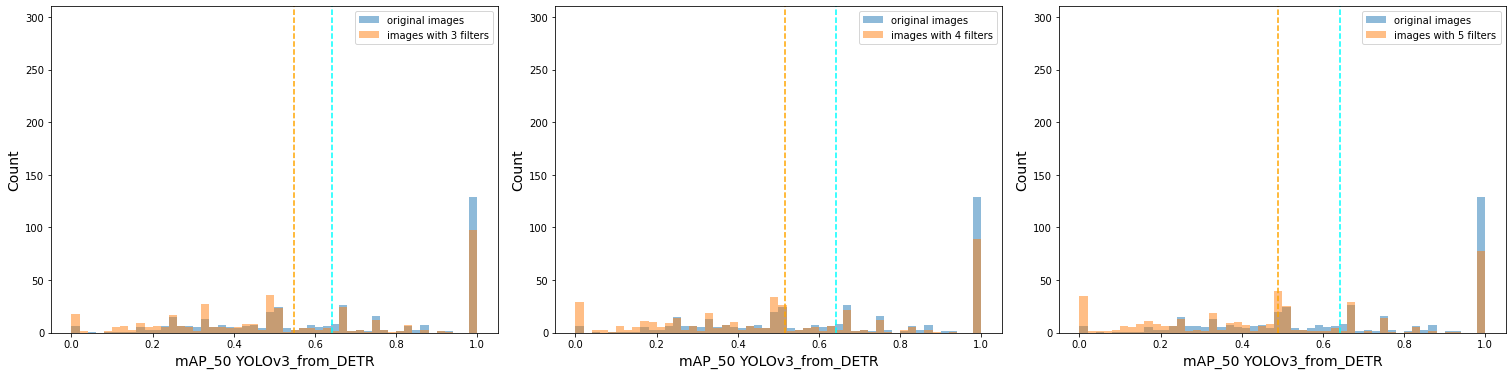
\includegraphics[width=1\textwidth]{Experiments/imgs/y3d.png}
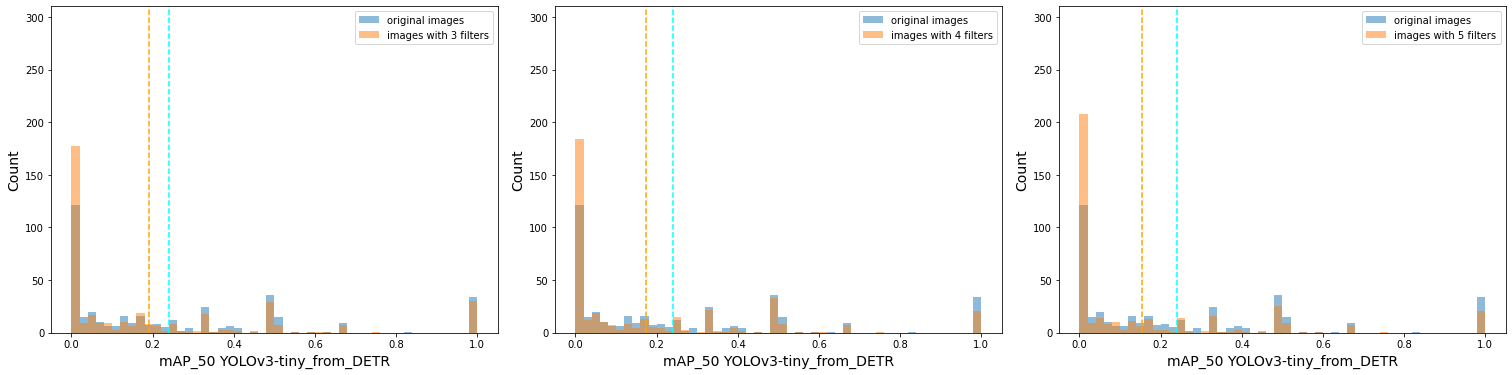
\includegraphics[width=1\textwidth]{Experiments/imgs/y3td.png}
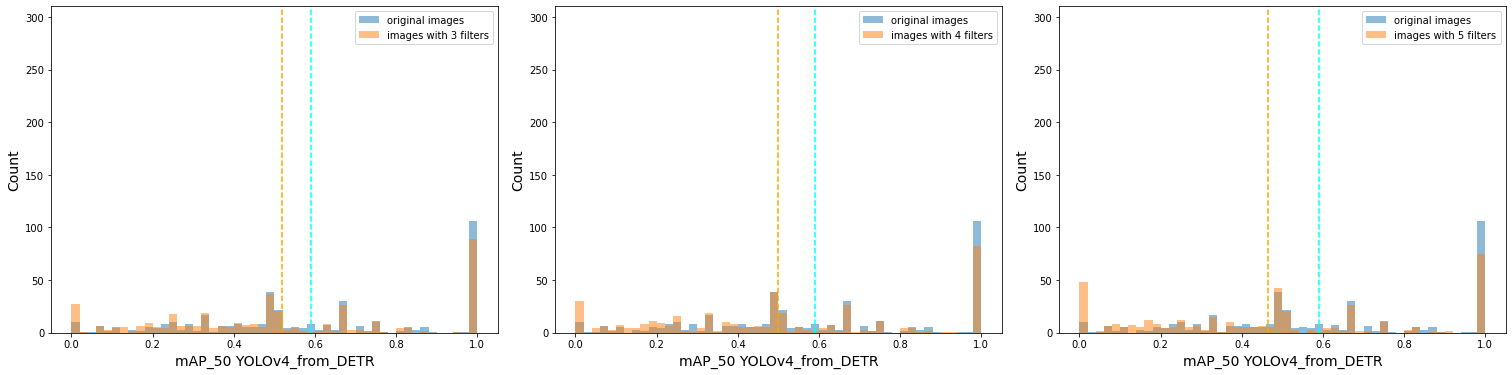
\includegraphics[width=1\textwidth]{Experiments/imgs/y4d.png}
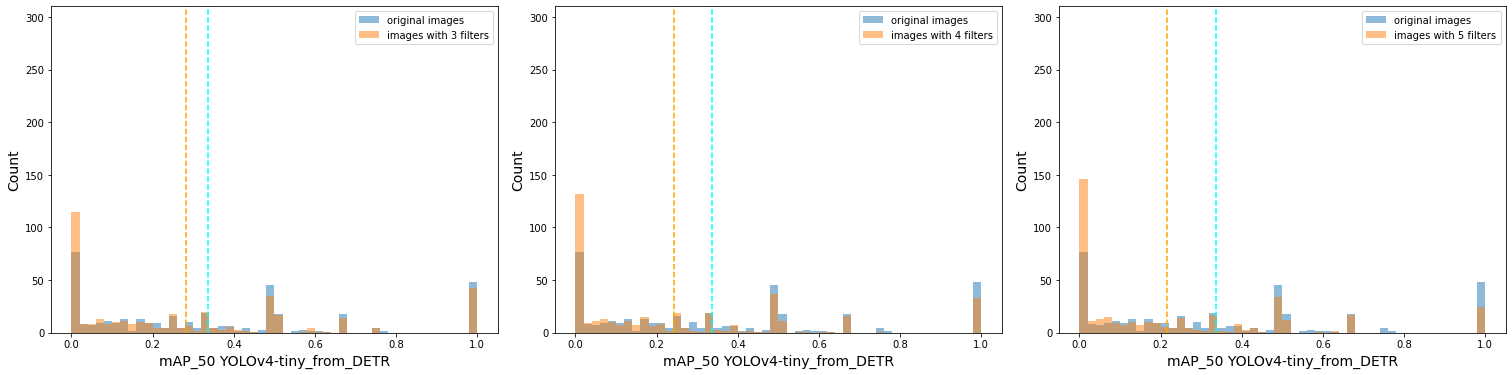
\includegraphics[width=1\textwidth]{Experiments/imgs/y4td.png}
\caption{Distribution of mAP\_50 values obtained on YOLOv3, YOLOv3-tiny, YOLOv4, YOLOv4-tiny from DETR-optimized filters. The vertical blue dotted line represents the mean over all the mAP\_50 values of the original images. The orange one represents the mean over all the mAP\_50 values of the filtered images}
\label{hysto_transfer}
\end{figure}

\begin{table}[H]\caption{YOLO and DETR Attack results. Precision and Recall values are calculated with IOU threshold 0.5.\\
In BRISQUE, the lower the score, the better the image quality should be (↓). \\In NIMA, the higher the score, the better the image quality should be (↑).}
\label{tab_transfer}
\resizebox{\textwidth}{!}{%
\begin{tabular}{llllllllll}
\hline
\multicolumn{10}{c}{\textbf{YOLOv3 (with DETR filters)}} \\ \hline
 & mAP & mAP\_50 & mAP\_75 & precision & recall & SSIM↑ & NIMA↑ & BRISQUE↓ &  \\ \cline{2-9}
no filters & 0.32 & 0.51 & 0.35 & 0.53 & 0.53 & 1.00 & 5.07 & 51.49 &  \\
3 filters & 0.26 (-19\%) & 0.41 & 0.28 & 0.39 & 0.43 & 0.85 & 4.77 & 57.28 &  \\
4 filters & 0.25 (-22\%) & 0.40 & 0.27 & 0.35 & 0.41 & 0.82 & 4.76 & 57.51 &  \\
5 filters & 0.22 (-31\%) & 0.36 & 0.25 & 0.30 & 0.30 & 0.78 & 4.74 & 57.67 &  \\ \hline
\end{tabular}%
}
\end{table}


\begin{table}[H]
\resizebox{\textwidth}{!}{%
\begin{tabular}{llllllllll}
\hline
\multicolumn{10}{c}{\textbf{YOLOv3-tiny (with DETR filters)}} \\ \hline
 & mAP & mAP\_50 & mAP\_75 & precision & recall & SSIM↑ & NIMA↑ & BRISQUE↓ &  \\ \cline{2-9}
no filters & 0.10 & 0.18 & 0.11 & 0.07 & 0.18 & 1.00 & 5.07 & 51.49 &  \\
3 filters & 0.08 (-27\%) & 0.13 & 0.07 & 0.03 & 0.13 & 0.85 & 4.77 & 57.28 &  \\
4 filters & 0.07 (-32\%) & 0.12 & 0.08 & 0.03 & 0.12 & 0.82 & 4.76 & 57.51 &  \\
5 filters & 0.06 (-39\%) & 0.11 & 0.07 & 0.03 & 0.11 & 0.78 & 4.74 & 57.67 &  \\ \hline
\end{tabular}%
}
\end{table}

\begin{table}[H]
\resizebox{\textwidth}{!}{%
\begin{tabular}{llllllllll}
\hline
\multicolumn{10}{c}{\textbf{YOLOv4 (with DETR filters)}} \\ \hline
 & mAP & mAP\_50 & mAP\_75 & precision & recall & SSIM↑ & NIMA↑ & BRISQUE↓ &  \\ \cline{2-9}
no filters & 0.34 & 0.47 & 0.38 & 0.47 & 0.49 & 1.00 & 5.07 & 51.49 &  \\
3 filters & 0.29 (-13\%) & 0.41 & 0.32 & 0.39 & 0.43 & 0.85 & 4.77 & 57.28 &  \\
4 filters & 0.28 (-18\%) & 0.38 & 0.31 & 0.30 & 0.40 & 0.82 & 4.76 & 57.51 &  \\
5 filters & 0.24 (-27\%) & 0.34 & 0.28 & 0.25 & 0.36 & 0.78 & 4.74 & 57.67 &  \\ \hline
\end{tabular}%
}
\end{table}

\begin{table}[H]
\resizebox{\textwidth}{!}{%
\begin{tabular}{llllllllll}
\hline
\multicolumn{10}{c}{\textbf{YOLOv4-tiny (with DETR filters)}} \\ \hline
 & mAP & mAP\_50 & mAP\_75 & precision & recall & SSIM↑ & NIMA↑ & BRISQUE↓ &  \\ \cline{2-9}
no filters & 0.15 & 0.24 & 0.17 & 0.16 & 0.25 & 1.00 & 5.07 & 51.49 &  \\
3 filters & 0.11 (-23\%) & 0.19 & 0.13 & 0.08 & 0.19 & 0.85 & 4.77 & 57.28 &  \\
4 filters & 0.10 (-32\%) & 0.16 & 0.11 & 0.05 & 0.16 & 0.82 & 4.76 & 57.51 &  \\
5 filters & 0.09 (-42\%) & 0.14 & 0.09 & 0.04 & 0.14 & 0.78 & 4.74 & 57.67 &  \\ \hline
\end{tabular}%
}
\end{table}

\begin{figure}[h]% 
    \centering
    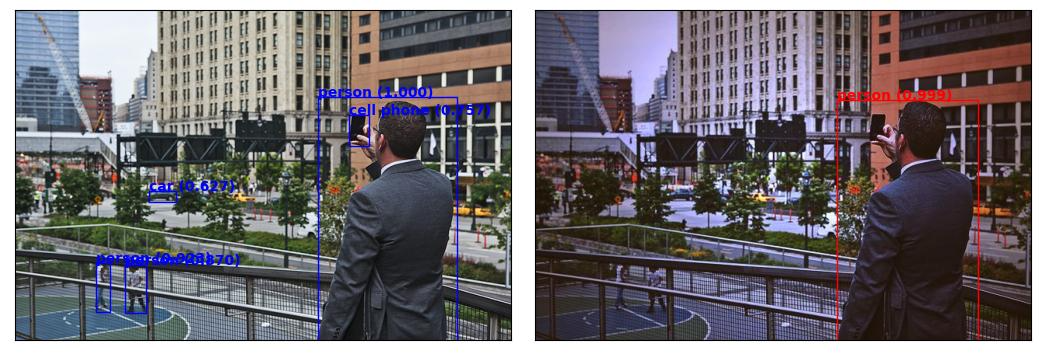
\includegraphics[width=0.85\textwidth]{Experiments/imgs/0.8_545100.png}
    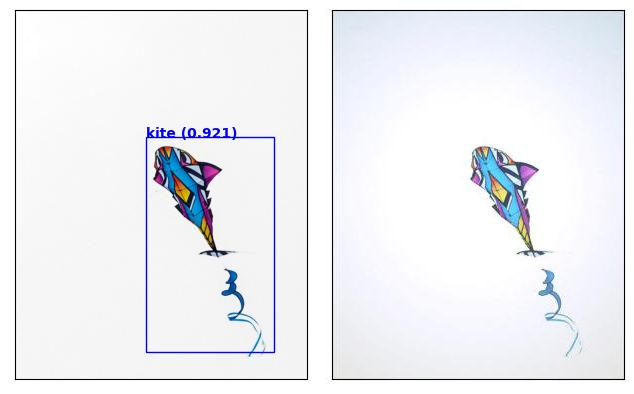
\includegraphics[width=0.85\textwidth]{Experiments/imgs/1_85665.png}
    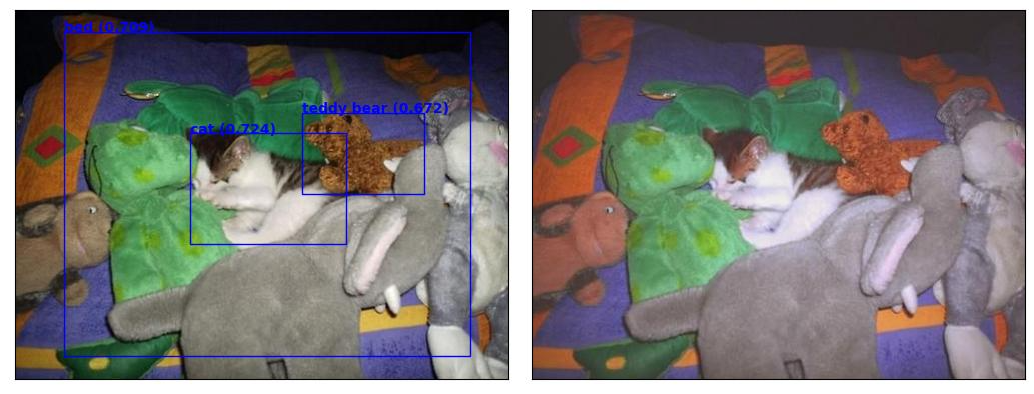
\includegraphics[width=0.85\textwidth]{Experiments/imgs/1_434996.png}
    \caption{On the left: images without filters and YOLOv3 detected bounding-boxes (in blue). On the right: images with 4 adversarial filters and YOLOv3 detected bounding-boxes (in red).}
    \label{fig:objdet_samples}
\end{figure}

\begin{figure}[h]% 
    \centering
    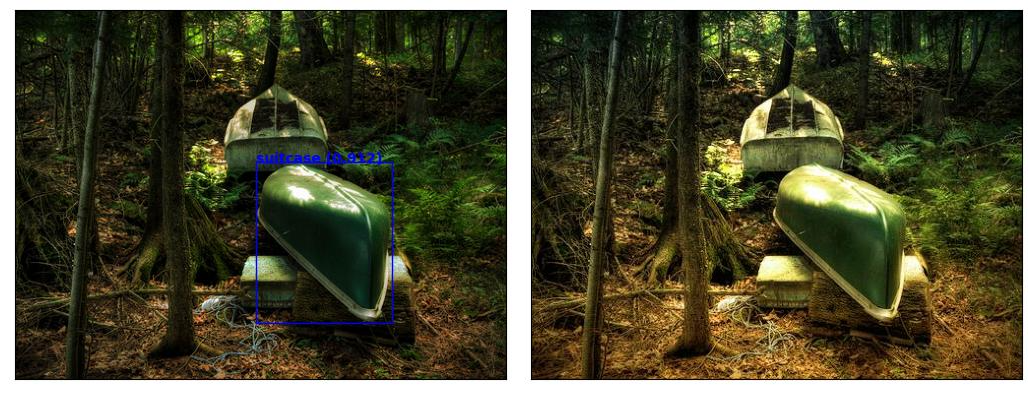
\includegraphics[width=0.85\textwidth]{Experiments/imgs/imgdetr1.png}
    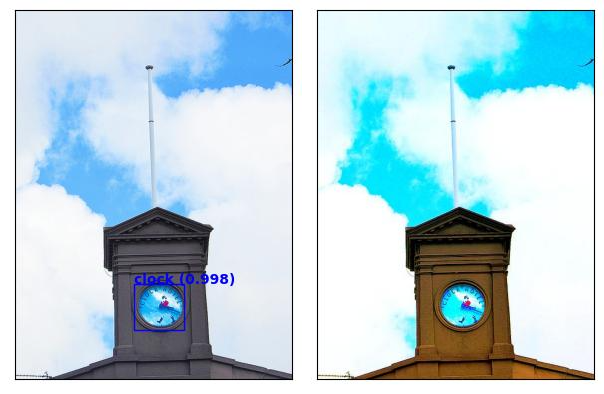
\includegraphics[width=0.85\textwidth]{Experiments/imgs/imgdetr2.png}
    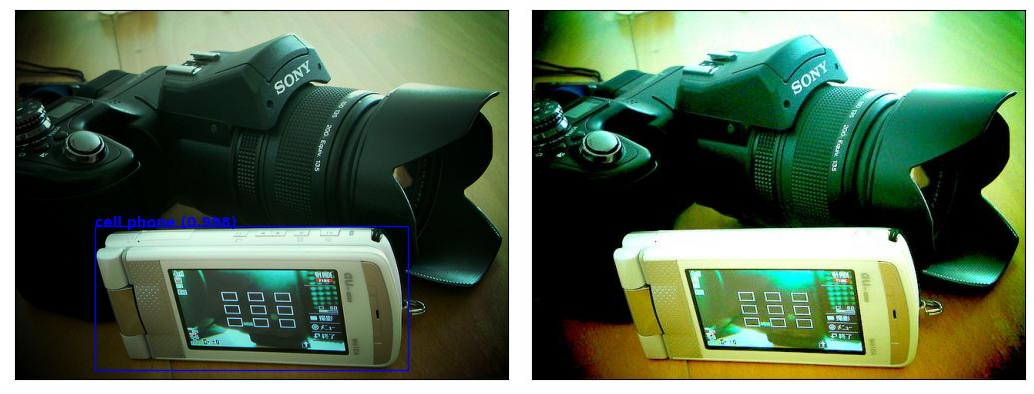
\includegraphics[width=0.85\textwidth]{Experiments/imgs/imgdetr4.png}
    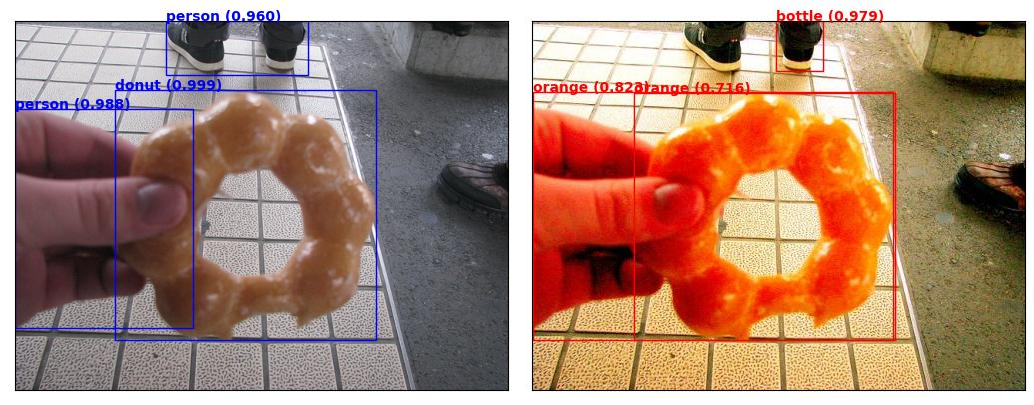
\includegraphics[width=0.85\textwidth]{Experiments/imgs/imgdetr5.png}
    \caption{On the left: images without filters and DETR detected bounding-boxes (in blue). On the right: images with 3 adversarial filters and DETR detected bounding-boxes (in red).}
    \label{fig:objdet_samples_detr}
\end{figure}

\begin{figure}[h]
    \centering
    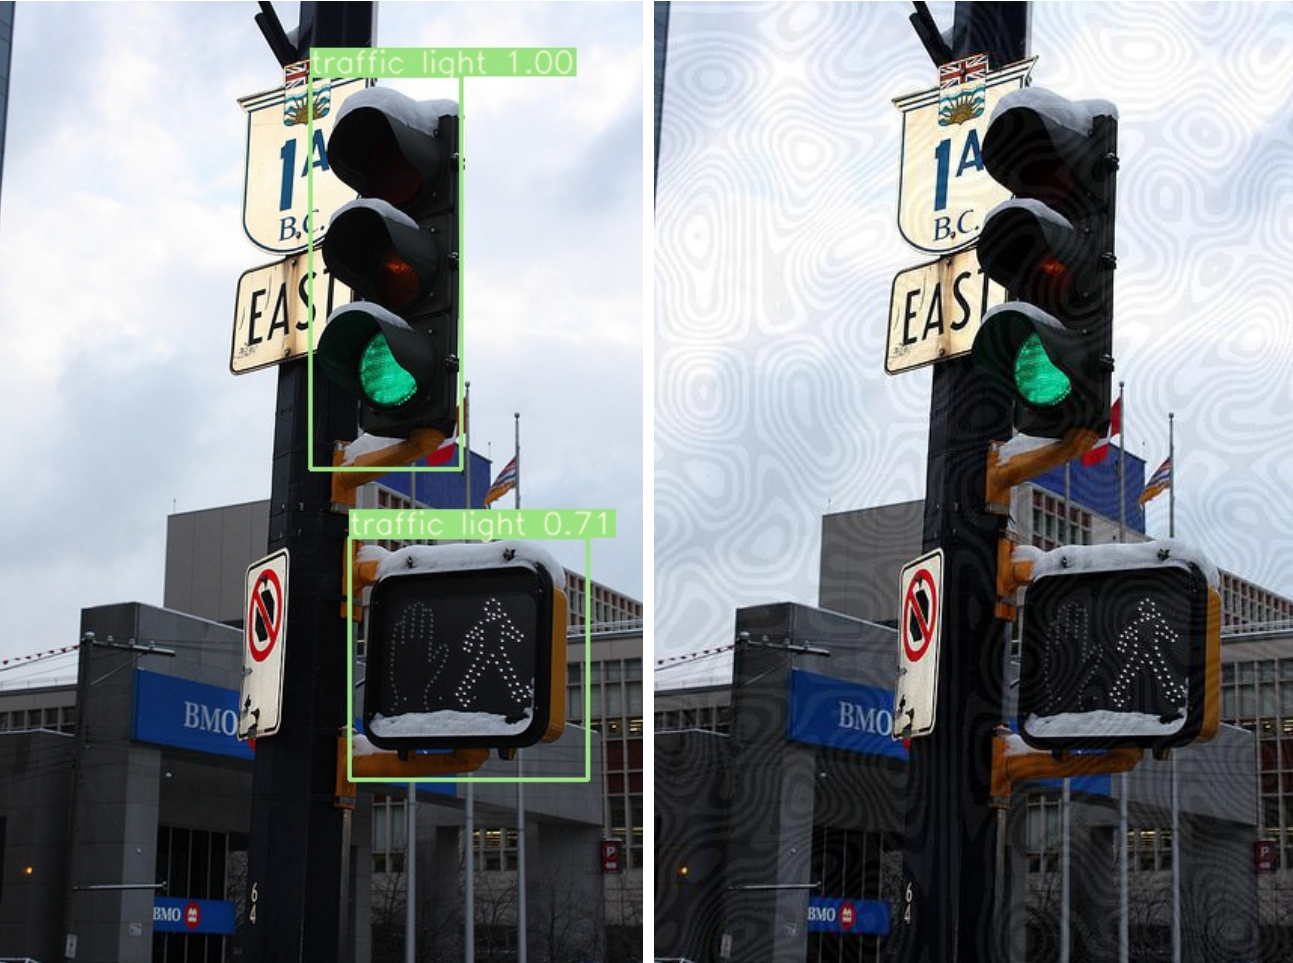
\includegraphics[width=0.8\textwidth]{Experiments/imgs/semaforo.png}
    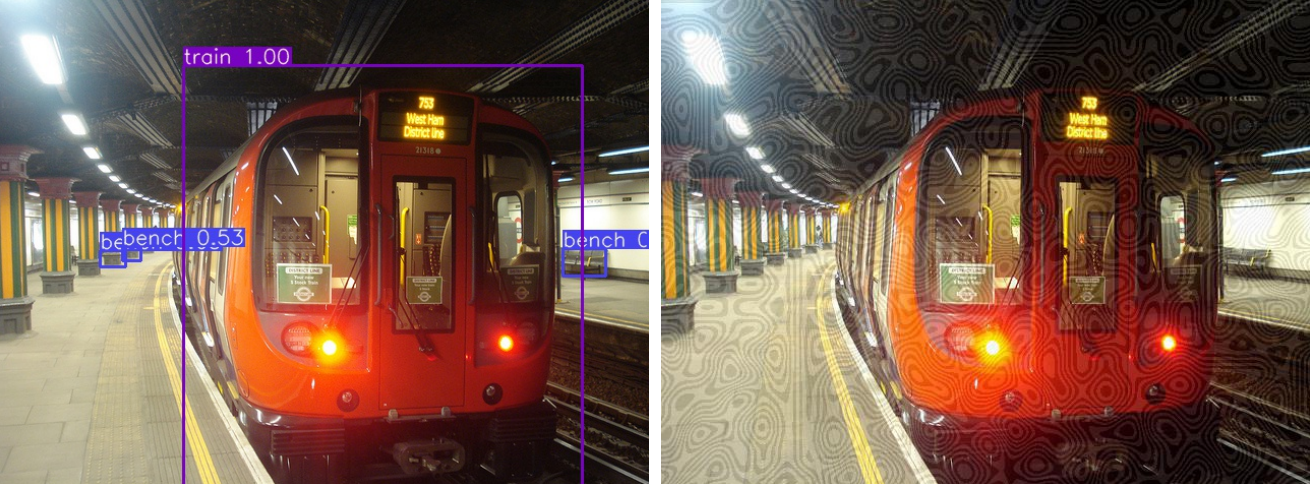
\includegraphics[width=0.8\textwidth]{Experiments/imgs/treno.png}
    \caption{Perlin noise adversarial examples on YOLO v3 from \cite{procNoise_co2019}}
    \label{fig:procnoise_samples}
\end{figure}





\chapter*{Conclusion}

In this thesis we studied, analyzed and tested the applicability of the AGV algorithm with respect to different object detection models.  To obtain the adversarial perturbation, popular Instagram-like image filters were optimized by employing a multi-objective evolutionary approach and these filters were applied across the entire image in order to generate the adversarial examples.  The optimization process considers both an object detection performance (ODP) and an image quality assessment index (SSIM) when searching for the optimal perturbation. \\


 The new version of the AGV algorithm was empirically evaluated on different state-of-the-art object detectors. As the results show, the method is able to generate natural-looking and artifacts-free adversarial samples that can effectively decrease the task performance of the tested models, resulting in successful attacks. \\

%{\bf Due parole sulla transferability. Verificare se negli altri paper citati è mai stata studiata.}

Results also show that AGV attacks can be transferable between various detector architectures.
This makes it particularly practical to implement real-world attacks. For instance, the filters that are optimized for lowering DETR performance can effectively attack YOLO as shown in Fig \ref{hysto_transfer} 


%{\bf Due parole sull'analisi della qualità delle immagini risultanti. Oltre ad essere artifacts-free per natura la qualità misurata con le più note misure risulta molto alta o addirittura migliore dell'originale secondo BRISQUE.}

Our research suggests that AGV can execute successful attacks in a "blackbox" environment, i.e., without being aware of the characteristics and designs of the targeted network and unlike patch-based and perturbation-based attacks AGV generates nice and natural looking adversarial images.
%This is also shown by the table \ref{tab_transfer} where



\noindent Moreover, the attack can be considered very efficient because the number of queries needed to perform it is relatively small considering the limited knowledge and access to the target models.


%{\it vedere se si riesce a trovare un termine di paragone}

The effective implementation of AGV also demonstrates the present detector architectures inherent susceptibility to these kinds of filter-based adversarial attacks.




 


\printbibliography[title={Bibliography}]
\addcontentsline{toc}{chapter}{Bibliography}

\end{document}
